\documentclass[11pt,a4paper,UTF8]{ctexart}

\usepackage[margin=0.85in]{geometry}
\usepackage{amsmath,amssymb,amsthm}
\usepackage{booktabs}
\usepackage{graphicx}
\usepackage{xcolor}
\usepackage{enumitem}
\usepackage{hyperref}
\usepackage{fancyhdr}
\usepackage{float}

\hypersetup{
  colorlinks=true,
  linkcolor=blue!60!black,
  citecolor=blue!60!black,
  urlcolor=blue!60!black
}

\newtheorem{proposition}{命题}
\newtheorem{definition}{定义}

\pagestyle{fancy}
\fancyhf{}
\setlength{\headheight}{14pt}
\lhead{炼钢厂钢包周转与同轨行车排产优化（中文对照版）}
\rhead{第 \thepage 页}
\renewcommand{\headrulewidth}{0.4pt}

\begin{document}

% ============================================================================
% 一页执行摘要（Summary Sheet 中文对照）
% ============================================================================
\thispagestyle{empty}
\begin{center}
  {\Large \textbf{炼钢—精炼—连铸过程多台同轨行车钢包吊运安全时空协同调度}}\\[0.25em]
  {\normalsize \textit{执行摘要（中文审阅版）}}
\end{center}
\vspace{0.1em}
\hrule
\vspace{0.4em}
{\small
\noindent\textbf{工业背景与数据取证诊断。}
在集成化炼钢—精炼—连铸（SCC）车间中，盛装高温钢水的钢包需要在转炉（BOF）、二次精炼（LF、RH）与连铸机（CCM）之间由共享同一轨道的桥式行车往返吊运。通过对 12 份真实车间工作簿（17.5 天、6,758 条原始行；1,321 条出钢计划含 55 条 \texttt{-2} 占位行与 1,266 条有效计划炉次、152 个连连浇号）进行非破坏性取证审计，我们发现\emph{工序间排队等待而非行车纯运输}主导全流程周期：静态计划内嵌了 15--30~min 的固定转运缓冲，而干净实测记录中出钢、LF、RH、连铸的中位纯时长分别为 5.63、36.92、39.00 与 40.65~min；浇次 \texttt{6C0754} 的实测相邻炉开浇间隔压缩至 1.53--2.78~min。审计同时标出 2,529 条待复核异常候选——包括综合表 72 组重复熔炼号、RH 表 533 行脱气起止相等记录、\texttt{3\#LF} 323 行吊起缺失，以及连铸下线空包重量高达 137.0--149.9~t（直接解释了现场 150~t 行车被绕开、主要由 450~t 行车吊运的原因）。

\noindent\textbf{统一框架与场景 1（确定性基准）。}
沿图 1 核验的 E--F 跨西东物理顺序 $\text{2\#150} \prec \text{4\#450} \prec \text{3\#450} \prec \text{5\#450} \prec \text{1\#150}$，我们构建了“炉次事件网络 + 单轨不可跨越行车调度”统一模型，完整覆盖四类耦合任务：重包前向运输（405.5--421.3~t）、连铸后空包回程（直落/翻渣/铸余回收分支落至 \texttt{1\#--3\#} 过渡平车）、C 炉专属空包上钢包车以及双炉关联铸余回收。在“安全可行与连续浇铸 $\succ$ 最小炉次等待 $\succ$ 最小行车运行时间”的词典序目标下，我们证明了匀速分段线性轨迹在所有折点满足间距约束等价于全连续时间防碰撞。在浇次 \texttt{6C0754}（6 炉、18 项主任务）历史回放中，\texttt{3\#450} 承担 116.87~min 作业（\texttt{5\#450} 为 72.40~min、\texttt{4\#450} 仅 14.35~min），开浇延误从 $-0.93$~min 漂移至 $+19.00$~min，热龄由 9.98~min 升至 31.72~min。切换到统一 \texttt{ef-initial-v1} 运动学配置（$D=12.0$~m、零切换时间）后，启用主动避让将总待吊时间从最优单机串行的 7.50~min 降至 \textbf{0.52~min}（\textbf{$-93.1\%$}，18/18 完成、0 迟到、最小间距 12.24~m），而关闭避让则在 1/18 处即死锁。在全量 17.5 天 ETL（843/1,321 = 63.8\% 唯一匹配炉次、3,764 条运输任务）上，常规日（2026-09-28，197 任务）与峰值日（2026-10-02，287 任务）预约调度均实现 100\% 覆盖与 12.5~m 安全间距，且证实保留东侧 2--3 条平车轨显著优于增设第 4 轨或将 \texttt{CART3} 西移（西移至 90~m 使峰值日等待由 1,158.1 飙升至 2,154.2~min）。

\noindent\textbf{场景 2（多档位变速与随机工时）。}
针对随机工序时间、有限加减速、离散档位与设备降速区，我们建立前向—后向 $v^2(x)$ 速度包络与日块乘性抽样—非预见性滚动 $\text{SAA-CVaR}_\alpha$ 框架 \cite{rockafellar2000optimization}。在 100 组独立随机情景下，自适应滚动派车使平均迟到下降 \textbf{74.4\%--84.6\%}（09-28：100.01 $\rightarrow$ 25.59~min；10-02：293.13 $\rightarrow$ 45.22~min），CVaR90 迟到下降 \textbf{61.1\%--78.4\%}（309.95 $\rightarrow$ 120.55~min；937.15 $\rightarrow$ 202.18~min），09-28 零迟到率从 0\% 升至 39\%。

\noindent\textbf{场景 3（故障重调度与恢复边界）。}
我们将扰动划分为微扰动（10~min 就绪延迟）与四类宏故障（转炉、LF/RH、连铸、行车/断轨） \cite{liu2021ladle}，并证明了行车故障下的轨道拓扑分割条件。8 类静态持久障碍压力测试表明，\texttt{4\#450} 停摆导致的任务服务率跌幅最大（46.2\%/47.7\%），其次为中区断轨（70.1\%/70.7\%）与 \texttt{3\#450}（75.1\%/79.4\%），而工位类故障均维持 100\% 服务覆盖；跨区 LF/RH 替代因增加 $>60$~min 迟到违约而被否决。

\noindent\textbf{独立验证与管理建议。}
场景 1 全部轨迹通过独立黑盒连续时间防碰撞核验（12.24--12.50~m 间距、0 碰撞）。条件性管理建议包括：保持平车东侧集聚、150~t 行车两端待命、优先保障 \texttt{4\#450} 可用性及升级 MES 双主键关联。

\vspace{0.3em}
\begin{table}[H]
\centering
\footnotesize
\caption*{三场景核心指标汇总}
\resizebox{\textwidth}{!}{%
\begin{tabular}{lccc}
\toprule
\textbf{评价指标} & \textbf{场景 1（确定性基准）} & \textbf{场景 2（随机与变速）} & \textbf{场景 3（故障恢复）} \\
\midrule
样本 / 范围 & \texttt{6C0754} 单浇次 / 整日预约 & 100 组随机日块情景 & 8 类故障压力情景 \\
等待 / 迟到 & 0.52~min（6C0754）；474.0/1,156.2~min（2轨整日） & 均值 25.59/45.22~min（-74\% 至 -85\%） & 工位故障 100\% 服务；\texttt{4\#450} 46.2\% \\
安全校验 & 12.24--12.50~m $\ge$ 12~m（0 碰撞） & 时间风险代理；制动包络已验证 & 0 碰撞；L1 恢复已验证 \\
\bottomrule
\end{tabular}%
}
\end{table}
}
\newpage

\tableofcontents
\newpage

% ============================================================================
% 第一章：引言
% ============================================================================
\section{引言}

\subsection{工业背景与运行瓶颈}
现代炼钢—精炼—连铸（SCC）车间是典型的批次—连续强耦合生产系统 \cite{tang2001review,tang2000mathematical,xuan2007scheduling,sun2025integrated}。转炉（BOF）冶炼出钢后的高温钢水注入钢包，按钢种要求进入钢包精炼炉（LF）或真空循环脱气装置（RH）精炼，再送往连铸机（CCM）连续浇铸成坯；浇毕后的空包经翻渣、铸余回收与热修后返回转炉循环使用。

在本研究工厂（图~\ref{fig:plant_layout}）中，E--F 跨共有 5 台共享同一轨道、且不可相互跨越的桥式行车：2 台额定 150~t（\texttt{1\#150}、\texttt{2\#150}）和 3 台额定 450~t（\texttt{3\#450}、\texttt{4\#450}、\texttt{5\#450}） \cite{peterson2014crane,zhu2006crane,lim2007mparallel,shin2026advances}。轨道干涉、空包回程拥堵与钢包车占用延迟直接威胁连铸不断浇与钢水热品质 \cite{li2020simulation}。

\begin{figure}[htbp]
  \centering
  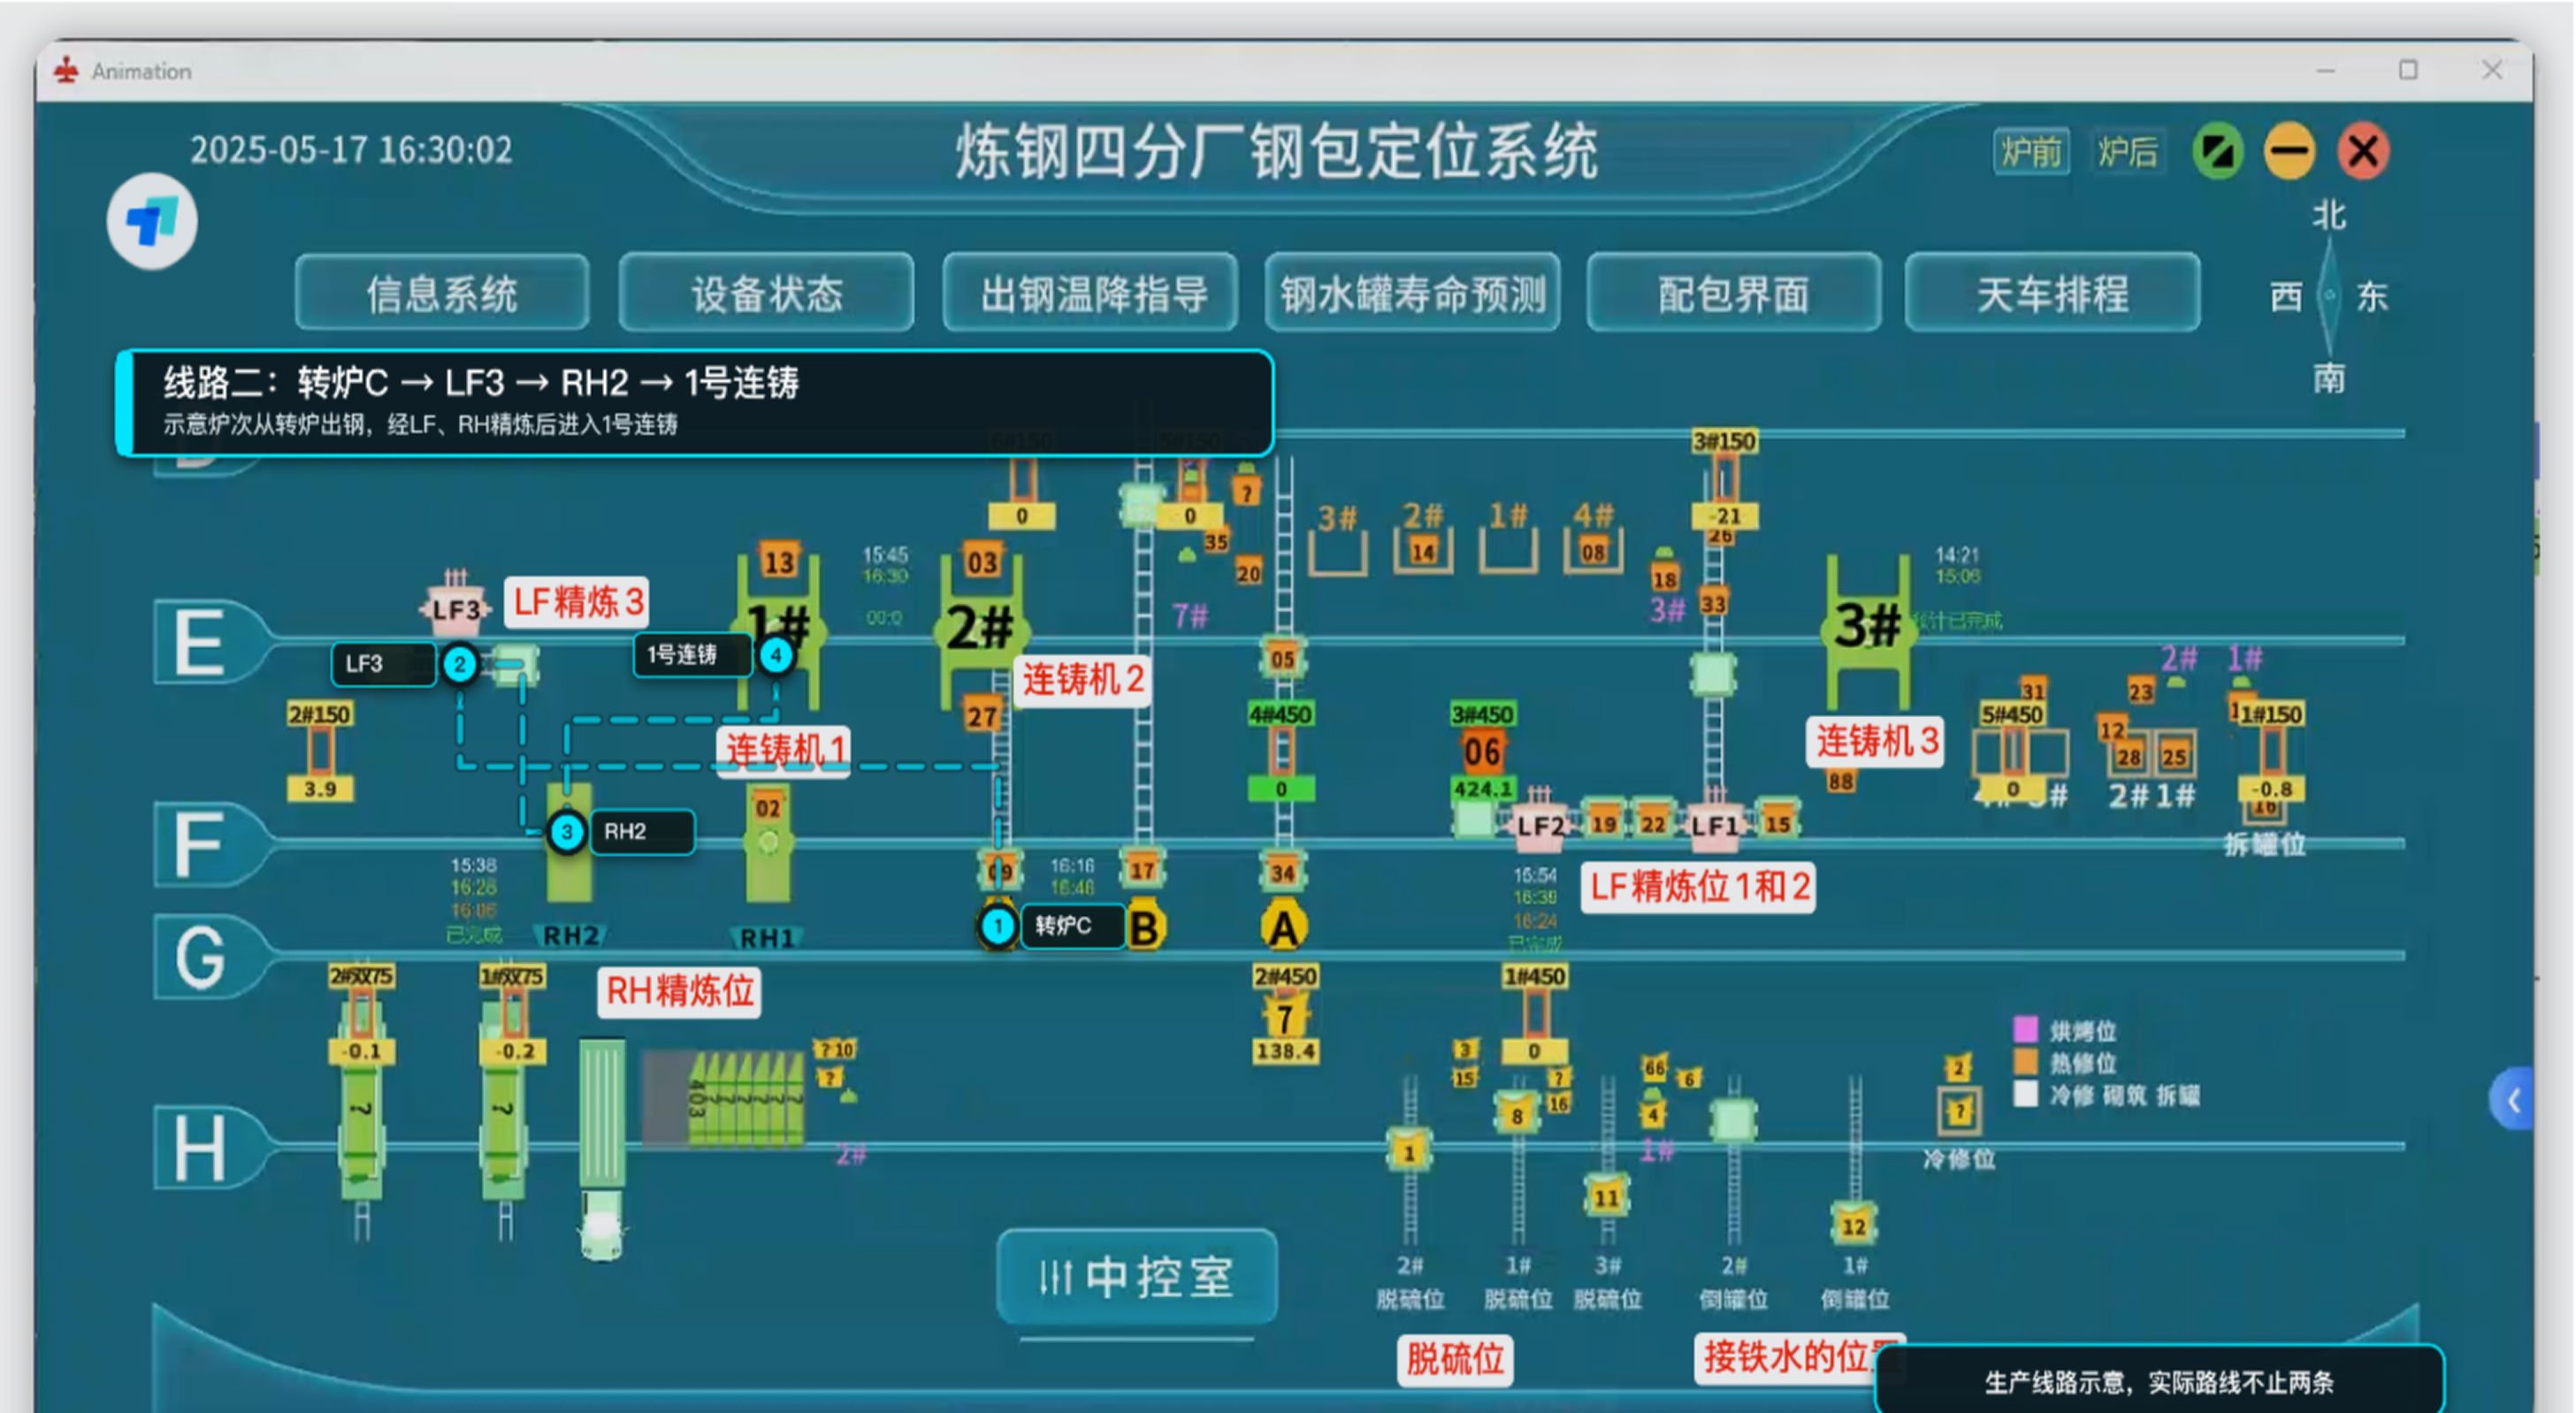
\includegraphics[width=0.95\textwidth]{figures/fig1_plant_layout_raw.png}
  \caption{炼钢四分厂设备与 E--F 跨五台行车物理布局示意图。}
  \label{fig:plant_layout}
\end{figure}

\subsection{问题拆解与三场景统一架构}
题目要求在严格词典序下求解三类递增复杂度场景：（1）保证安全（零碰撞、零超载、不断浇）；（2）最小化炉次等待时间；（3）最小化行车运行时间。
\begin{itemize}[leftmargin=1.5em,itemsep=2pt]
  \item \textbf{场景 1（确定性基准）：} 工序时间确定、行车匀速运行、操作切换时间为零。
  \item \textbf{场景 2（随机工时与真实运动学）：} 工序时间服从随机分布，考虑加减速、多档位与特殊位置降速避让。
  \item \textbf{场景 3（故障触发重调度）：} 出钢及钢包车就绪延迟扰动与设备/行车故障下的保序恢复。
\end{itemize}

\begin{figure}[htbp]
  \centering
  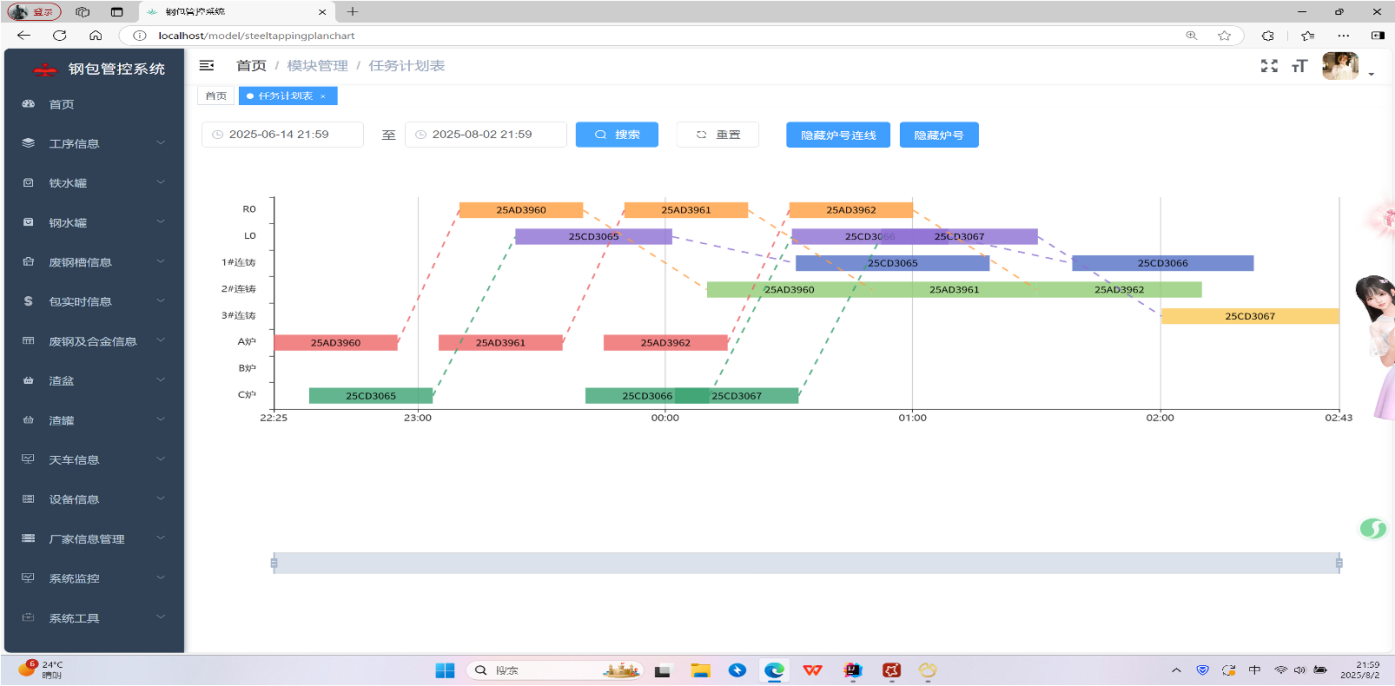
\includegraphics[width=0.90\textwidth]{figures/fig2_mes_gantt_raw.png}
  \caption{车间 MES 炉次流转甘特界面（展示 \texttt{L0}、\texttt{R0} 精炼路径与跨工序转运连线）。}
  \label{fig:mes_gantt}
\end{figure}

% ============================================================================
% 第二章：多源数据取证与实证诊断
% ============================================================================
\section{多源数据取证与实证诊断}

\subsection{12 份生产工作簿的非破坏性审计}
我们对《出钢计划表单.xls》及 11 份设备工序表（时间跨度 2026-09-24 23:24 至 2026-10-12 13:04，共 6,758 条原始行）进行了全量 SHA-256 登记与非破坏性质量扫描。由于 6 份 \texttt{.xlsx} 表存在 XML 维度头误写为 \texttt{A1} 的问题，解析时采用全表正常模式。核心实证结论如下：
\begin{enumerate}[leftmargin=1.5em,itemsep=2pt]
  \item \textbf{有效计划分母：} 1,321 条原始计划中含 55 条 \texttt{配包flag = -2} 占位行，有效计划炉次为 \textbf{1,266 炉}、对应 \textbf{152 个连连浇号}；有效行中 $(\texttt{更换中包} == 1) \Leftrightarrow (\texttt{浇次号} == 1)$ 严格一致（205 条，0 错配）。
  \item \textbf{四类精炼路线分布：} \texttt{L0}（仅 LF，668 炉，52.8\%）、\texttt{R0}（仅 RH，420 炉，33.2\%）、\texttt{R0L0}（RH$\rightarrow$LF，108 炉，8.5\%）、\texttt{L0R0}（LF$\rightarrow$RH，70 炉，5.5\%）。
  \item \textbf{复合主键必要性：} 计划表中熔炼号唯一，但《工序时间信息.xlsx》（1,355 行）存在 \textbf{72 组重复熔炼号}（144 行）绑定不同钢包与错开时间戳。因此必须采用 \texttt{(熔炼号, 物理钢包号)} 与 \texttt{临时罐号} 联合关联。
  \item \textbf{非破坏性异常保留（2,529 条复核候选）：} 两 RH 表有 533 行脱气起止时刻相等（改用 \texttt{RH处理周期} 口径）；\texttt{3\#LF} 缺 323 行吊起时刻与车号；\texttt{B炉} 缺 435 行钢水罐临时号；四组时序存在负差候选（113、115、143、238 行），均完整保留标记而不强行截零。
\end{enumerate}

\subsection{计划与实测工时对比及行车载荷不对称性}
表~\ref{tab:duration_stats} 与图~\ref{fig:data_audit} 对比了计划名义时长与干净实测记录。计划赋予转炉恒定 30.0~min 时槽，而实测出钢中位仅 5.63~min。同时，数据揭示了关键的物理不对称性：
\begin{itemize}[leftmargin=1.5em,itemsep=2pt]
  \item \textbf{E--F 跨西东物理序：} 图 1 实测排序为 $\text{2\#150} \prec \text{4\#450} \prec \text{3\#450} \prec \text{5\#450} \prec \text{1\#150}$，与编号顺序不同。
  \item \textbf{为何现场绕开 150~t 行车：} 重包总重达 395--421.3~t；连铸下线空包因含残钢残渣，重量达 137.0--150.9~t，频繁逼近甚至超过 150~t 红线，因此 E--F 跨实测任务全部由 3 台 450~t 行车承担。
\end{itemize}

\begin{table}[htbp]
\centering
\small
\caption{全量有效炉次计划与干净实测工序时长统计（\texttt{basic\_duration\_stats.csv}）}
\label{tab:duration_stats}
\resizebox{\textwidth}{!}{%
\begin{tabular}{llrrrrrr}
\toprule
\textbf{工序 / 指标} & \textbf{路线} & \textbf{$n_{\text{clean}}$} & \textbf{均值 (min)} & \textbf{标准差 (min)} & \textbf{P10 (min)} & \textbf{中位数 (min)} & \textbf{P90 (min)} \\
\midrule
计划转炉 & ALL & 1,266 & 30.00 & 0.00 & 30.00 & 30.00 & 30.00 \\
实测出钢 & ALL & 1,065 & 5.74 & 1.42 & 4.47 & 5.63 & 7.23 \\
实测 LF 处理 & ALL & 751 & 38.49 & 13.19 & 28.72 & 36.92 & 47.68 \\
实测 RH 处理 & ALL & 516 & 38.64 & 8.01 & 28.46 & 39.00 & 47.41 \\
计划浇铸 & ALL & 1,266 & 41.03 & 3.30 & 37.00 & 40.00 & 46.00 \\
实测浇铸 & ALL & 1,117 & 41.45 & 5.00 & 36.23 & 40.65 & 47.89 \\
\bottomrule
\end{tabular}%
}
\end{table}

\begin{figure}[htbp]
  \centering
  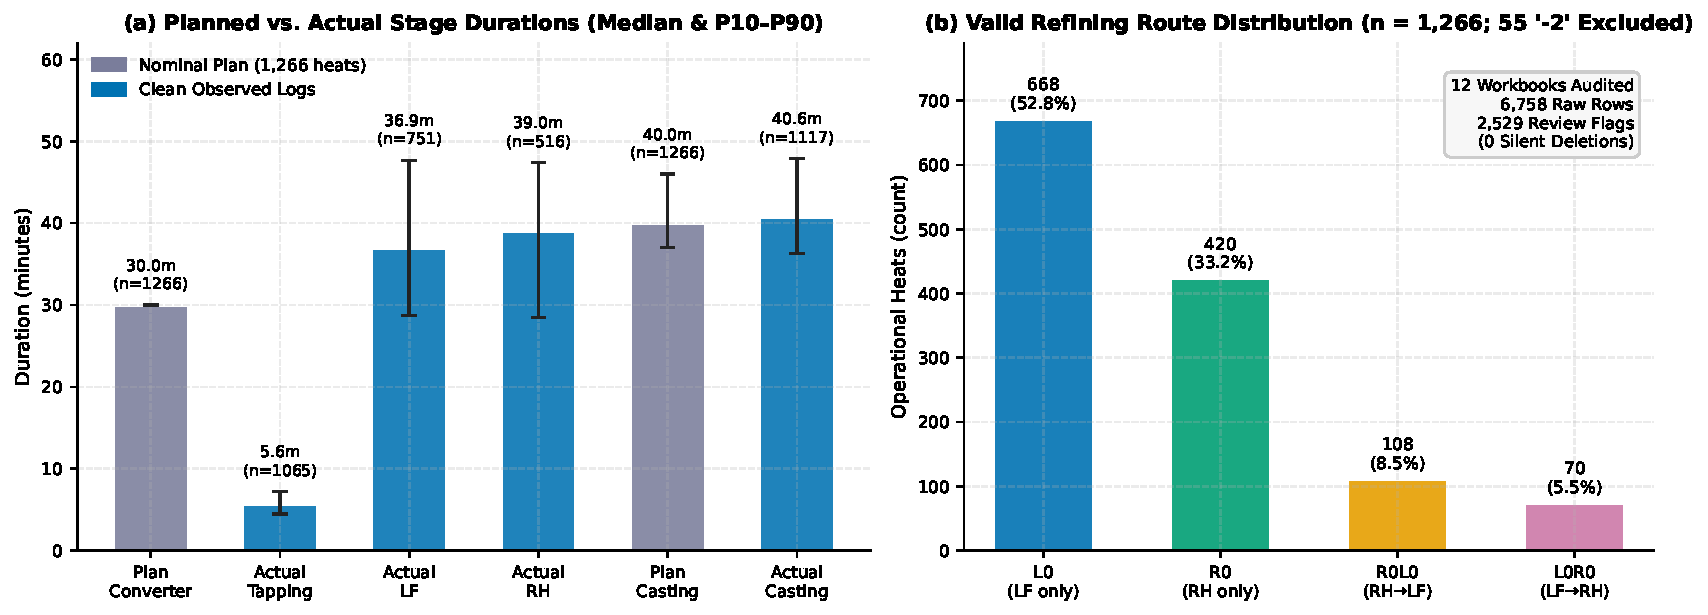
\includegraphics[width=0.96\textwidth]{figures/fig3_data_audit_durations.pdf}
  \caption{(a) 1,266 炉次计划与实测工序时长中位数及 P10--P90 区间；(b) 精炼路线构成与 12 表审计总量。}
  \label{fig:data_audit}
\end{figure}

% ============================================================================
% 第三章：模型假设、符号与统一时空数学模型
% ============================================================================
\section{模型假设、符号体系与统一时空模型}

\subsection{核心模型假设}
\begin{enumerate}[leftmargin=1.5em,itemsep=2pt]
  \item \textbf{钢包数量充足：} 遵循题设（26 个钢包循环），不因缺包取消炉次，优化聚焦行车响应性与连铸连续性。
  \item \textbf{单轨不可跨越约束：} E--F 跨 5 台行车共享一维轨道 $x \in [0, L]$（$L=240$~m），始终保持西东顺序 $k \in \{1,\dots,5\}$。
  \item \textbf{载荷兼容约束：} 仅当总吊重 $w_j \le W_k^{\max}$ 时允许行车 $k$ 吊运任务 $j$（150~t 辅车正式门槛为 145~t）。
  \item \textbf{过渡平车布局假设：} 按题面与图 1，在 E--F 跨东侧设置 3 条空包过渡平车轨（\texttt{CART1}--\texttt{CART3}，单轨容量 1 罐），并在第 4/7 节进行数量与西移灵敏度分析。
  \item \textbf{双工位与滞留占用：} LF/RH 区分接受位与处理位，但处理完成后的钢包在吊离前仍占据工位。
\end{enumerate}

\subsection{核心符号表与四类任务拆解}
表~\ref{tab:nomenclature} 汇总了三场景共用的集合、参数与决策变量。E--F 跨行车任务集 $J$ 拆分为四类：（1）\textbf{重包前向运输}（单精炼 2 段、双精炼 3 段）；（2）\textbf{连铸后空包回程}（直落平车、翻渣后落平车、铸余回收分支）；（3）\textbf{C 炉专属平车供包}（\texttt{C\_IN\_h}，A/B 炉经 D--E 跨衔接）；（4）\textbf{双炉关联铸余回收}（通过 \texttt{recovery\_id} 绑定供余与接收炉次）。

\begin{table}[htbp]
\centering
\small
\caption{三场景统一模型核心符号表}
\label{tab:nomenclature}
\begin{tabular}{llp{8.4cm}}
\toprule
\textbf{符号} & \textbf{类型} & \textbf{物理含义与单位} \\
\midrule
$K = \{1,\dots,5\}$ & 集合 & 按西东序排列的 5 台 E--F 跨行车：\texttt{2\#150, 4\#450, 3\#450, 5\#450, 1\#150} \\
$J, H, M$ & 集合 & 吊运任务集（$J$）、有效炉次集（$H$）、设备与平车集（$M$） \\
$o_j, d_j \in [0, L]$ & 参数 & 任务 $j$ 起点与终点的轨道坐标（m；$L=240$~m） \\
$r_j, b_j, w_j$ & 参数 & 任务 $j$ 最早可吊时刻（s）、截止时刻（s）与总吊重（t） \\
$W_k^{\max}, D_k$ & 参数 & 额定吊重（150/450~t；辅车门槛 145~t）与相邻中心安全间距（12~m） \\
$a_j, c_j, \Delta_{\text{therm}}^{\max}$ & 参数 & 起落钩服务时长（s）与末道精炼结束至开浇热窗上限（1,800~s） \\
$S_{ho}, C_{ho}$ & 变量 & 炉次 $h$ 工序 $o$ 的开始与结束时刻（s） \\
$u_j, v_j, x_{jk}$ & 变量 & 任务 $j$ 的起吊时刻（s）、落包时刻（s）及行车指派变量（0--1） \\
$q_k(t), v_k(t)$ & 变量 & 行车 $k$ 在时刻 $t$ 的连续轨道位置（m）与速度（m/s） \\
\bottomrule
\end{tabular}
\end{table}

\subsection{核心时空安全约束}
\begin{align}
  u_j &\ge r_j, \qquad \sum_{k \in K_j} x_{jk} = 1, \\
  v_j &= u_j + a_j + T_k(o_j, d_j) + c_j \quad (\text{当 } x_{jk} = 1), \\
  S_{h,o+1} &\ge v_j \quad (\text{紧邻前序转运完成后方可开始下道工序}), \\
  u_j &\ge v_i + T_k^{\text{empty}}(d_i, o_j) \quad (\text{同车连续任务 } i \to j), \\
  q_{k+1}(t) - q_k(t) &\ge D_k \quad \forall t \ge 0,\; k \in \{1,\dots,4\}.
\end{align}

% ============================================================================
% 第四章：场景 1
% ============================================================================
\section{场景 1：确定性调度、\texttt{6C0754} 闭环与整日灵敏度}

\subsection{词典序目标与折点防碰撞充要性}
场景 1 极小化词典序目标 $\text{lex}\min\big(\text{Violations},\; \sum_j (u_j - r_j),\; R\big)$，其中 $R$ 为重载与空驶/避让总运行时间。
\begin{proposition}[匀速分段线性轨迹的折点防碰撞充要条件]
记 $\mathcal{T}$ 为全厂所有行车轨迹折点（空驶启停、起吊、落包、避让端点）的并集。在分段匀速假设下，$q_{k+1}(t)-q_k(t) \ge D_k$ 对任意连续时刻 $t$ 成立，当且仅当其在所有折点 $t \in \mathcal{T}$ 处成立。
\end{proposition}
\begin{proof}
在任意两个相邻折点开区间 $(t_m, t_{m+1})$ 内，$q_k(t)$ 与 $q_{k+1}(t)$ 均为仿射函数，其差值亦为仿射函数，故最小值必在端点 $t_m$ 或 $t_{m+1}$ 处取得。
\end{proof}

\subsection{浇次 \texttt{6C0754} 历史回放基准}
在 \texttt{6C0754}（6 炉 \texttt{26BD6452}--\texttt{26BD6457}，均为 B 炉 $\rightarrow$ 1\#RH $\rightarrow$ 3\#连铸，18 项主任务）历史回放中（图~\ref{fig:replay_6c0754}），\texttt{3\#450} 承担 116.87~min 作业，而 \texttt{5\#450} 为 72.40~min、\texttt{4\#450} 仅 14.35~min；同时开浇延误从 $-0.93$~min 逐步累积至 $+19.00$~min，热龄由 9.98~min 攀升至 31.72~min。

\begin{figure}[htbp]
  \centering
  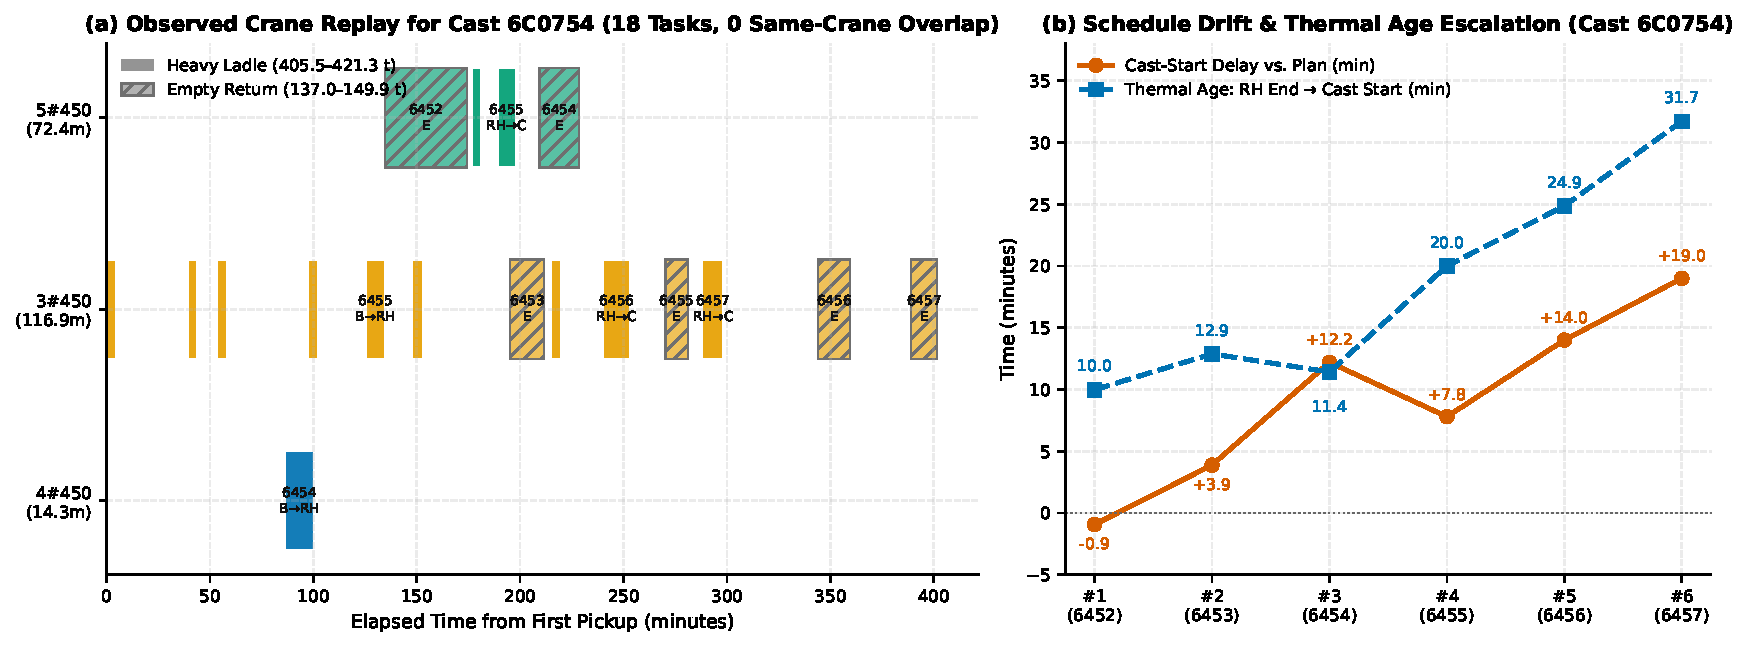
\includegraphics[width=0.96\textwidth]{figures/fig4_replay_6C0754_gantt.pdf}
  \caption{(a) 浇次 \texttt{6C0754} 实测行车任务甘特图；(b) 6 炉连续浇铸期间开浇延误与热龄爬升曲线。}
  \label{fig:replay_6c0754}
\end{figure}

\subsection{闭环轨道校验与“无避让必撞车”实证}
在临时像素配置下对 \texttt{6C0754} 开展 5 方案闭环对比（表~\ref{tab:closed_loop_6c0754}、图~\ref{fig:closed_loop_6c0754}），发现：
\begin{enumerate}[leftmargin=1.5em,itemsep=2pt]
  \item \textbf{无避让三机并行全部违约：} 历史回放、FCFS、EDF-Nearest 与 CP-SAT 精确空驶 \cite{ortools} 均发生 $-1{,}235$ 至 $-1{,}520$~px 的严重越界交叉；仅保守单机串行（\texttt{5\#450}）通过安全门禁（$+60.0$~px），但等待时间由 21.92~min 暴增至 109.48~min（多等 87.6~min）。
  \item \textbf{空包回程标定残差：} 连铸空包至平车实测中位耗时 16.02~min，而重包 OD 回归仅预测 3.41~min（残差 $+12.60$~min），证明必须将“站点翻渣/铸余作业时长”与“纯行车行驶时长”拆分建模。
\end{enumerate}

\begin{table}[htbp]
\centering
\small
\caption{浇次 \texttt{6C0754} 五方案闭环轨道安全对照（临时像素参数）}
\label{tab:closed_loop_6c0754}
\resizebox{\textwidth}{!}{%
\begin{tabular}{lrrrrrl}
\toprule
\textbf{调度策略} & \textbf{总等待 (min)} & \textbf{总迟到 (min)} & \textbf{跨度 (min)} & \textbf{最小间距 (px)} & \textbf{求解耗时 (s)} & \textbf{轨道门禁} \\
\midrule
历史实际回放 & 204.12 & 14.57 & 401.68 & $-1{,}235.0$ & --- & \textcolor{red!70!black}{违规} \\
FCFS（无避让） & 21.92 & 12.09 & 405.12 & $-1{,}520.0$ & --- & \textcolor{red!70!black}{违规} \\
EDF-Nearest（无避让） & 21.92 & 12.09 & 405.12 & $-1{,}235.0$ & --- & \textcolor{red!70!black}{违规} \\
CP-SAT（无避让） & 33.65 & 12.08 & 405.12 & $-1{,}520.0$ & 0.044 & \textcolor{red!70!black}{违规} \\
保守单机串行（\texttt{5\#450}） & 109.48 & 18.37 & 403.73 & $+60.0$ & 0.024 & \textcolor{green!50!black}{通过} \\
\bottomrule
\end{tabular}%
}
\end{table}

\begin{figure}[htbp]
  \centering
  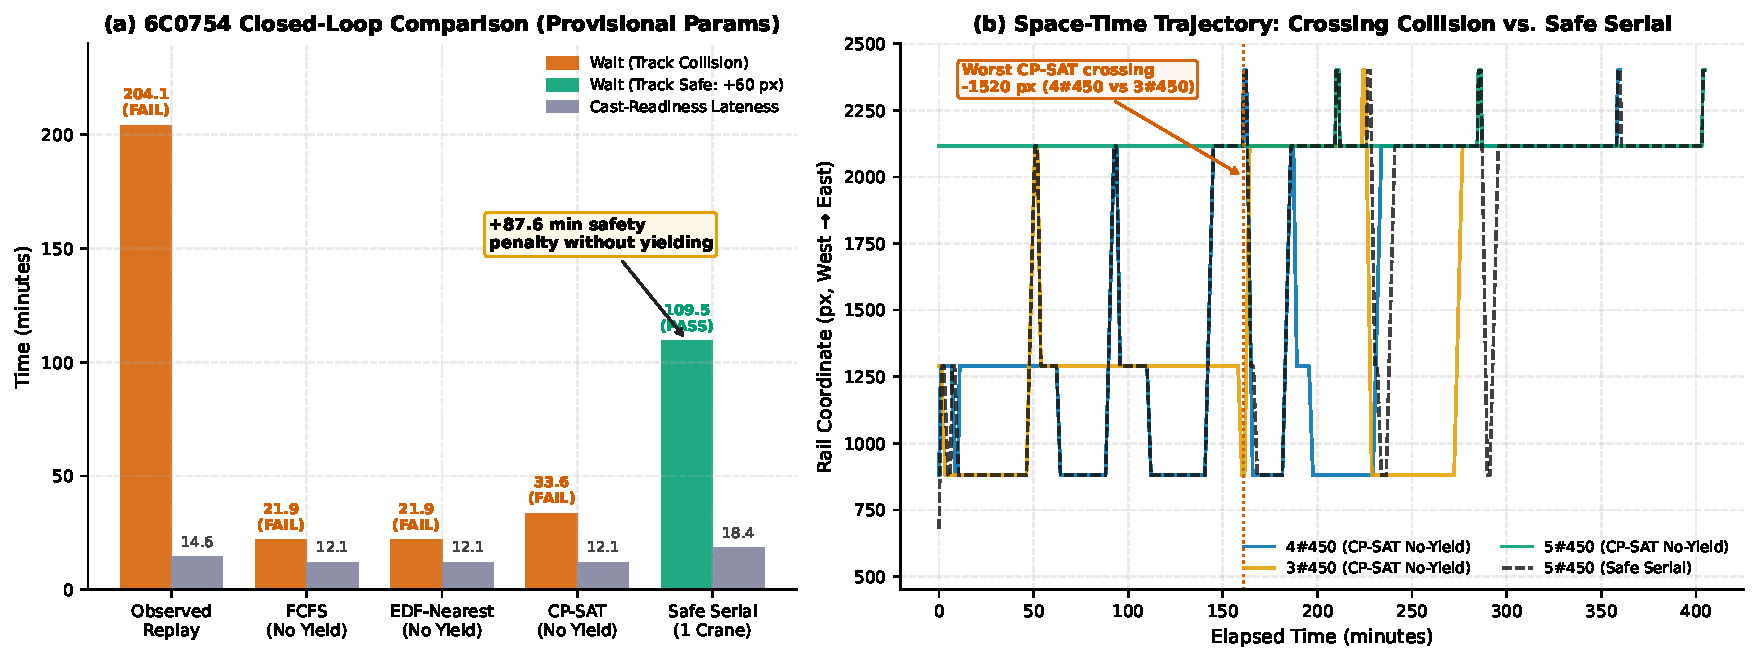
\includegraphics[width=0.96\textwidth]{figures/fig5_closed_loop_6C0754.pdf}
  \caption{(a) 5 方案等待、迟到与安全门禁对照；(b) CP-SAT 无避让交叉冲突轨迹 vs 保守单机安全包络。}
  \label{fig:closed_loop_6c0754}
\end{figure}

\subsection{基于 \texttt{ef-initial-v1} 的主动避让安全并行调度}
切换至正式米制配置 \texttt{ef-initial-v1}（$D=12.0$~m、速度 $0.60/0.80/1.00$~m/s、场景 1 零切换）并引入主动避让后（表~\ref{tab:yield_6c0754}、图~\ref{fig:yield_6c0754}）：\texttt{fcfs\_nearest} 完成全部 18 项任务、0 迟到、最小间距 12.24~m（$\ge 12.0$~m），总等待压至 \textbf{0.52~min}（较最优单机串行 7.50~min **降低 93.1\%**）；而关闭避让（\texttt{pipeline\_no\_yield}）在 1/18 处死锁，几何盲指派（\texttt{cp\_sat\_assignment}）触发 531 次避让并在 11/18 处死锁。

\begin{table}[htbp]
\centering
\small
\caption{浇次 \texttt{6C0754} 主动避让 vs 串行与死锁对照（\texttt{ef-initial-v1}, $D=12.0$~m）}
\label{tab:yield_6c0754}
\resizebox{\textwidth}{!}{%
\begin{tabular}{lcrrrrrl}
\toprule
\textbf{算法} & \textbf{完成数} & \textbf{总等待 (min)} & \textbf{迟到 (min)} & \textbf{避让次数} & \textbf{最小间距 (m)} & \textbf{使用行车} & \textbf{状态} \\
\midrule
\texttt{fcfs\_nearest}（主动避让） & 18/18 & \textbf{0.52} & 0.00 & 29 & 12.24 & \texttt{3\#450; 4\#450} & \textcolor{green!50!black}{通过} \\
\texttt{pipeline\_roles}（主动避让） & 18/18 & 3.30 & 0.00 & 11 & 12.35 & \texttt{3\#450; 4\#450} & \textcolor{green!50!black}{通过} \\
\texttt{serial\_4\#450} & 18/18 & 7.50 & 0.00 & 2 & 12.34 & \texttt{4\#450} & \textcolor{green!50!black}{通过} \\
\texttt{serial\_3\#450} & 18/18 & 8.32 & 0.00 & 2 & 12.40 & \texttt{3\#450} & \textcolor{green!50!black}{通过} \\
\texttt{serial\_5\#450} & 18/18 & 9.83 & 0.00 & 4 & 12.40 & \texttt{5\#450} & \textcolor{green!50!black}{通过} \\
\texttt{cp\_sat\_assignment} & 11/18 & 2.78 & 0.00 & 531 & 12.28 & \texttt{3\#/4\#/5\#450} & \textcolor{red!70!black}{死锁} \\
\texttt{pipeline\_no\_yield} & 1/18 & 0.52 & 0.00 & 0 & 12.40 & \texttt{4\#450} & \textcolor{red!70!black}{死锁} \\
\bottomrule
\end{tabular}%
}
\end{table}

\begin{figure}[htbp]
  \centering
  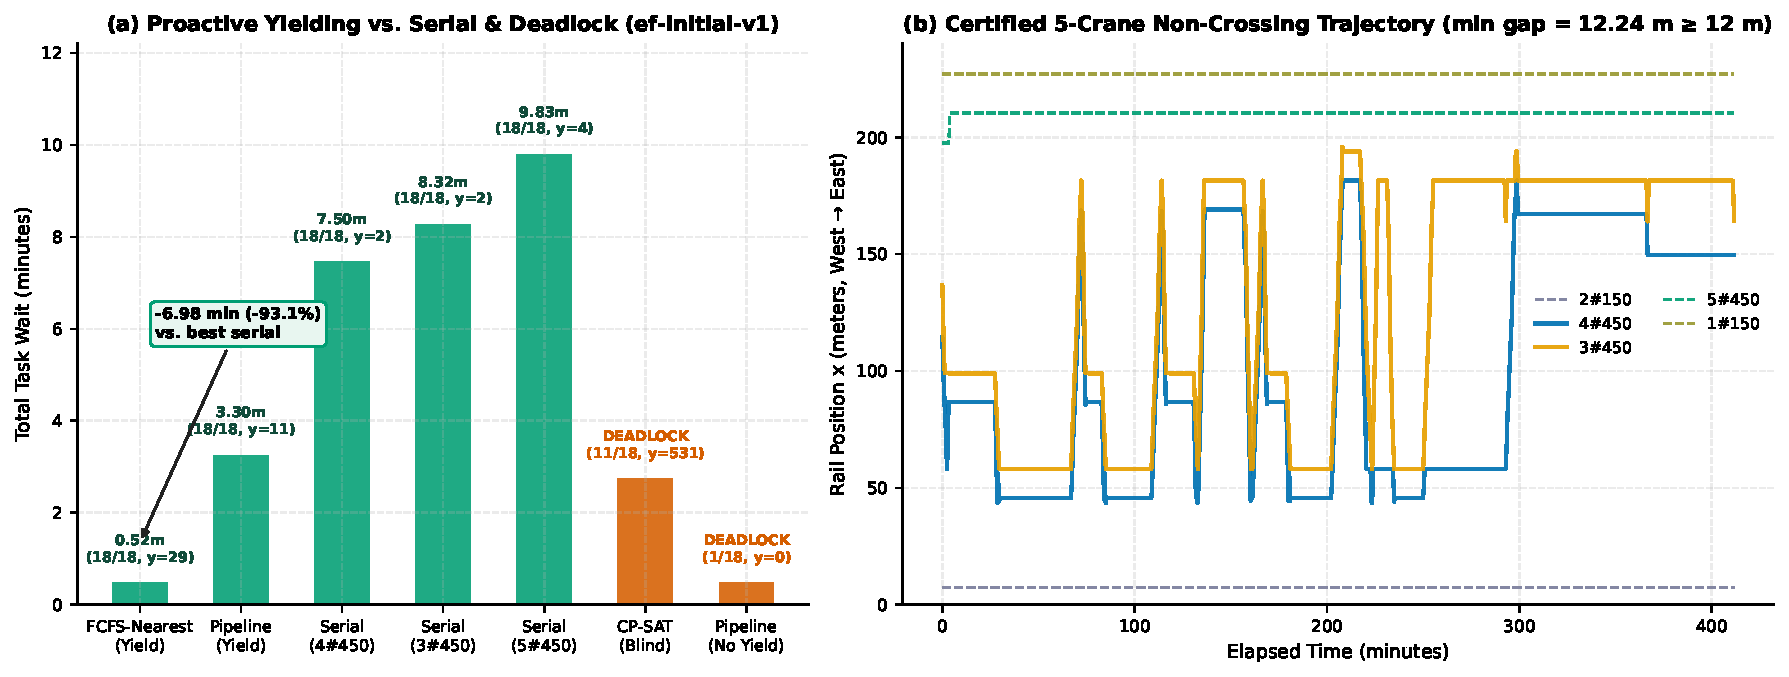
\includegraphics[width=0.96\textwidth]{figures/fig6_yield_6C0754.pdf}
  \caption{(a) 主动避让（0.52~min）与串行/死锁方案对比；(b) \texttt{fcfs\_nearest} 1 秒分辨率五车安全轨迹（最小间距 12.24~m $\ge$ 12.0~m）。}
  \label{fig:yield_6c0754}
\end{figure}

\subsection{整日多浇次调度、150~t 辅车边界与平车布局灵敏度}
全量 17.5 天 ETL 在 5,400~s / 3.0~t 契约下唯一匹配 \textbf{843 炉}（占 1,321 条计划的 63.8\%，3,407 道工序、3,764 条运输任务），选出常规日 \textbf{2026-09-28}（48 炉、197 任务）与峰值日 \textbf{2026-10-02}（59 炉、287 任务）。两日预约调度均实现 100\% 任务覆盖与 12.5~m 最小间距（表~\ref{tab:day_layout}、图~\ref{fig:day_layout_aux}；串行运动口径下跨度 25.64/26.13~h，等待值为保守上界）：
\begin{enumerate}[leftmargin=1.5em,itemsep=2pt]
  \item \textbf{平车东侧集聚显著优于西移与增轨：} 2 东轨（\texttt{COUNT\_2E}）与 3 东轨（\texttt{BASE\_3E}）在两日表现最优（09-28：474.0/476.0~min；10-02：1,156.2/1,158.1~min）；而增设第 4 轨（\texttt{COUNT\_4E}）或将 \texttt{CART3} 西移至 80/85/90~m 使峰值日等待恶化至 1,424.6 / 1,589.5 / 2,154.2~min（P95 达 24.3~min）。
  \item \textbf{150~t 辅车占位扫描：} 在 100/120/140/145~t 阈值下，峰值日 0 次启用，常规日仅接入 1 条 0~t 缺失重量占位任务（使等待升至 486.2~min）。该扫描属能力占位测试，正式定论需在补全正净重数据后重验。
\end{enumerate}

\begin{table}[htbp]
\centering
\scriptsize
\caption{整日过渡平车数量/选址与 150~t 辅车灵敏度（63.8\% 匹配口径；保守预约）}
\label{tab:day_layout}
\resizebox{\textwidth}{!}{%
\begin{tabular}{lrrrrrrr}
\toprule
\textbf{方案变体} & \textbf{日期 (09-28 / 10-02)} & \textbf{任务数} & \textbf{总等待 (min)} & \textbf{均值 (min)} & \textbf{P95 (min)} & \textbf{避让次数} & \textbf{最小间距 (m)} \\
\midrule
\texttt{COUNT\_2E}（2 东轨） & 09-28 / 10-02 & 197 / 287 & \textbf{474.0} / \textbf{1,156.2} & 2.41 / 4.03 & 8.9 / 13.6 & 112 / 146 & 12.5 / 12.5 \\
\texttt{BASE\_3E}（3 东轨） & 09-28 / 10-02 & 197 / 287 & 476.0 / 1,158.1 & 2.42 / 4.04 & 8.9 / 13.9 & 111 / 131 & 12.5 / 12.5 \\
\texttt{COUNT\_4E}（4 东轨） & 09-28 / 10-02 & 197 / 287 & 561.1 / 1,441.4 & 2.85 / 5.02 & 9.7 / 16.1 & 112 / 137 & 12.5 / 12.5 \\
\texttt{WEST\_3\_80}（80~m） & 09-28 / 10-02 & 197 / 287 & 475.0 / 1,424.6 & 2.41 / 4.96 & 8.9 / 17.5 & 105 / 128 & 12.5 / 12.5 \\
\texttt{WEST\_3\_85}（85~m） & 09-28 / 10-02 & 197 / 287 & 482.5 / 1,589.5 & 2.45 / 5.54 & 8.9 / 19.8 & 107 / 131 & 12.5 / 12.5 \\
\texttt{WEST\_3\_90}（90~m） & 09-28 / 10-02 & 197 / 287 & 496.7 / 2,154.2 & 2.52 / 7.51 & 9.4 / 24.3 & 108 / 133 & 12.5 / 12.5 \\
\texttt{AUX\_145t}（5 车对照） & 09-28 / 10-02 & 197 / 287 & 486.2 / 1,158.1 & 2.47 / 4.04 & 9.0 / 13.9 & 114 / 131 & 12.5 / 12.5 \\
\bottomrule
\end{tabular}%
}
\end{table}

\begin{figure}[htbp]
  \centering
  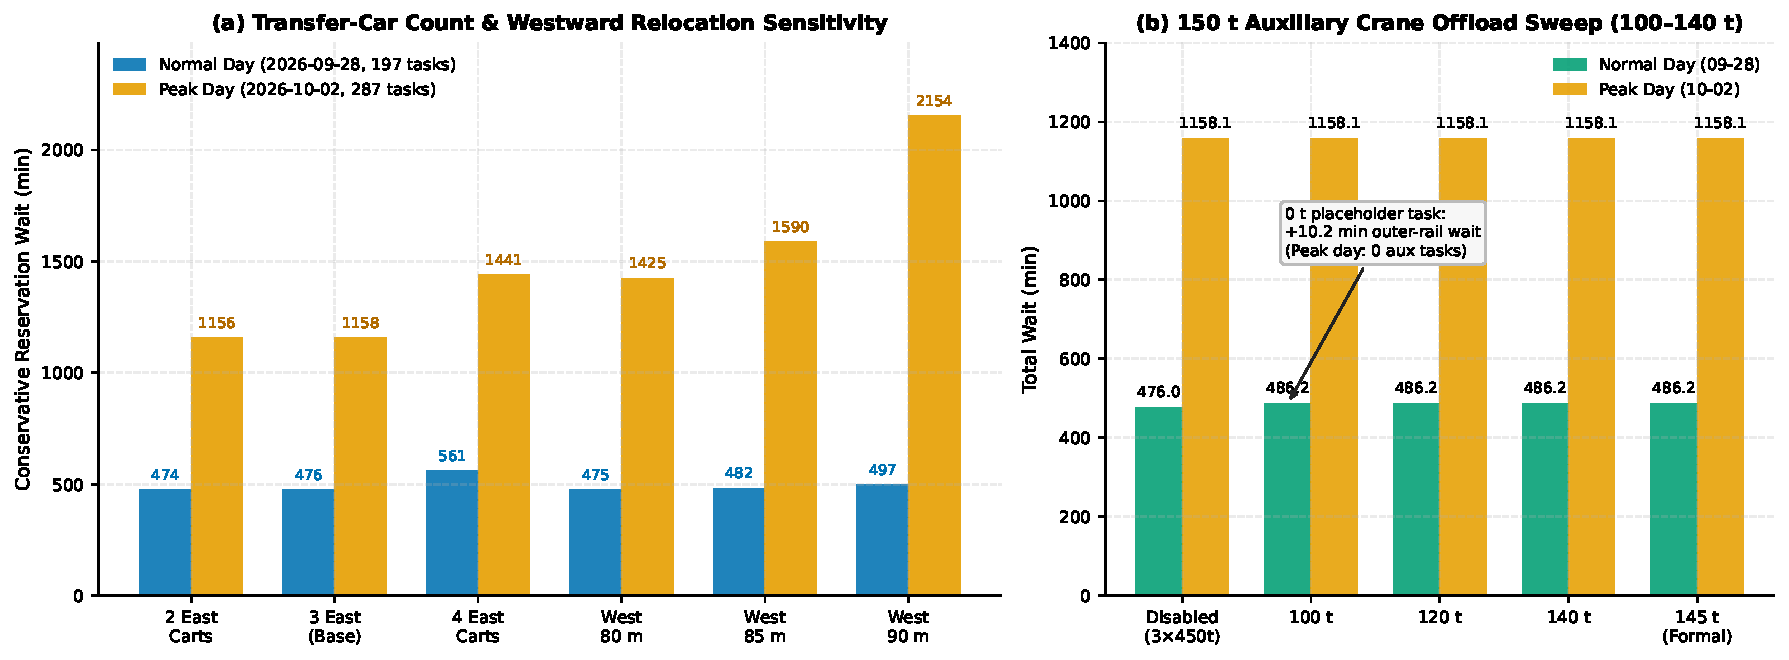
\includegraphics[width=0.96\textwidth]{figures/fig7_scene1_day_layout_aux.pdf}
  \caption{(a) 常规日与峰值日过渡平车数量及西移灵敏度；(b) 150~t 辅车阈值扫描。}
  \label{fig:day_layout_aux}
\end{figure}

% ============================================================================
% 第五章：场景 2
% ============================================================================
\section{场景 2：多档位变速运动学与风险厌恶随机调度}

\subsection{分段 $v^2(x)$ 速度包络运动学}
针对有限加减速 $a_k^+, a_k^-$、离散档位与设备降速区限速 $V_{\text{cap}}$，沿行驶距离 $\ell \in [0, |x_1-x_0|]$ 通过前向—后向平方速度包络计算可行最快轨迹：
\begin{align}
  (V_{i+1}^{f})^2 &= \min\big(V_{\text{cap}, i+1}^2,\; (V_i^f)^2 + 2a_k^+\delta\ell_i\big), \\
  (V_i^b)^2 &= \min\big((V_i^f)^2,\; (V_{i+1}^b)^2 + 2a_k^-\delta\ell_i\big).
\end{align}
单段包络诊断（\texttt{gear\_envelope\_2026-09-28.csv}）验证所有降速区均在入区前完成安全制动（重包 207.14~s vs 无约束 149.50~s；空包 154.72~s vs 113.12~s）。

\subsection{日块抽样与自适应时间风险评估}
基于拟合期日块乘性扰动与 100 组独立蒙特卡洛评价情景 \cite{kleywegt2002sample,ye2014robust,rockafellar2000optimization}（表~\ref{tab:scene2_risk}、图~\ref{fig:scene2_risk}）：零噪声退化与场景 1 基准（258.0/786.9~min）精确一致；自适应滚动派车较开环计划将平均迟到降低 \textbf{74.4\%--84.6\%}（100.01 $\rightarrow$ 25.59~min；293.13 $\rightarrow$ 45.22~min），CVaR90 尾均值降低 61.1\%--78.4\%。在同质日块冲击下，\texttt{rolling\_risk}（26.42/46.44~min）未超越 \texttt{rolling\_mean}，表明执行期实时反馈是主要收益来源。

\begin{table}[htbp]
\centering
\small
\caption{场景 2 时间风险代理评估（100 组独立抽样：开环计划 vs 自适应派车）}
\label{tab:scene2_risk}
\resizebox{\textwidth}{!}{%
\begin{tabular}{lrrrr}
\toprule
\textbf{策略} & \textbf{均值 (09-28 / 10-02)} & \textbf{P95 (09-28 / 10-02)} & \textbf{CVaR90 (09-28 / 10-02)} & \textbf{零迟到率 (09-28)} \\
\midrule
\texttt{mean\_plan}（开环） & 100.01 / 293.13 & 248.13 / 597.86 & 309.95 / 937.15 & 0.0\% \\
\texttt{conservative\_plan}（开环） & 98.83 / 293.13 & 245.34 / 597.86 & 306.16 / 937.14 & 0.0\% \\
\texttt{rolling\_mean}（自适应） & \textbf{25.59} / \textbf{45.22} & \textbf{93.65} / \textbf{152.01} & \textbf{120.55} / \textbf{202.18} & \textbf{39.0\%} \\
\texttt{rolling\_risk}（CVaR90） & 26.42 / 46.44 & 97.30 / 157.79 & 125.46 / 208.73 & 39.0\% \\
\bottomrule
\end{tabular}%
}
\end{table}

\begin{figure}[htbp]
  \centering
  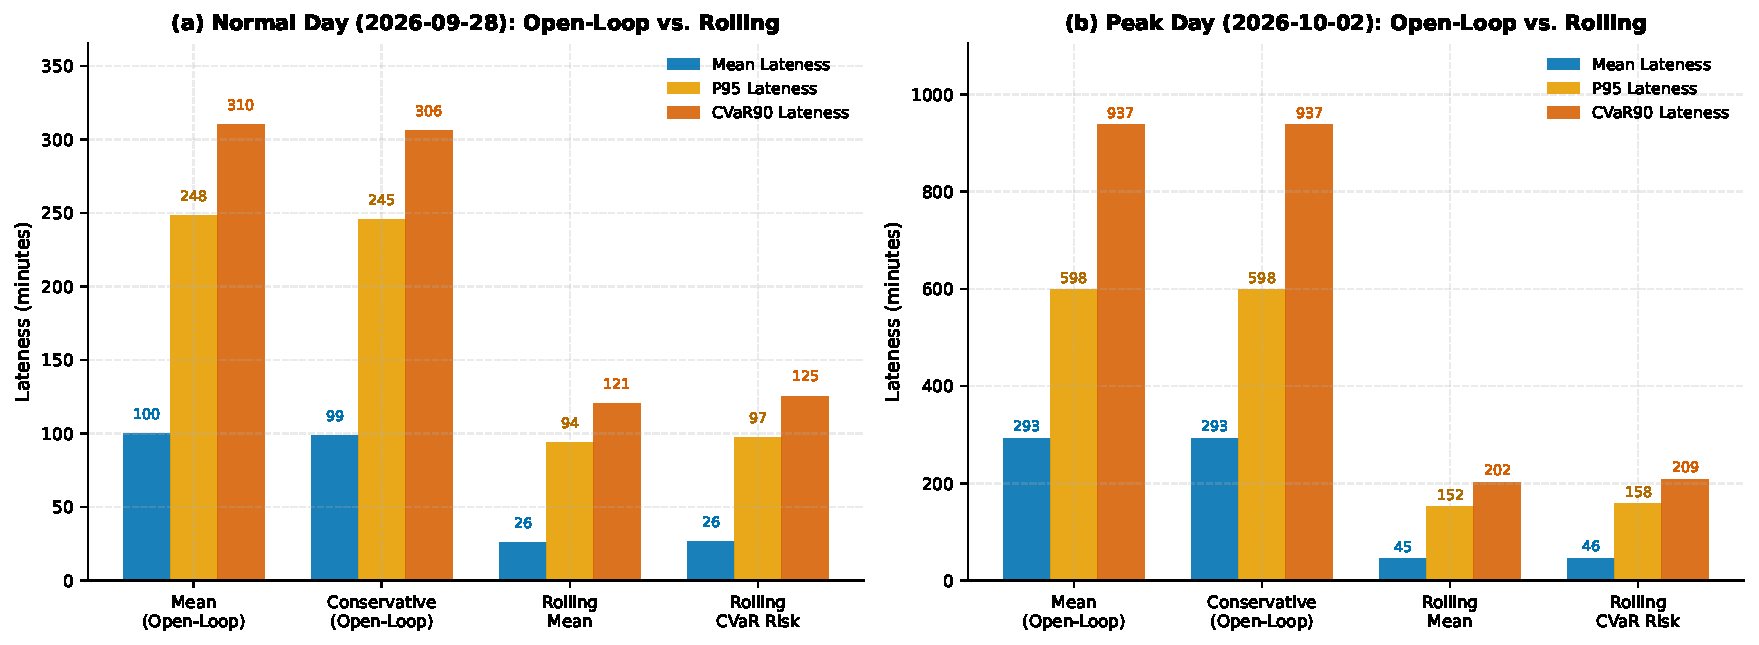
\includegraphics[width=0.96\textwidth]{figures/fig8_scene2_stochastic_risk.pdf}
  \caption{场景 2 开环计划与自适应滚动派车在 (a) 常规日与 (b) 峰值日上的均值、P95 与 CVaR90 迟到对比。}
  \label{fig:scene2_risk}
\end{figure}

% ============================================================================
% 第六章：场景 3
% ============================================================================
\section{场景 3：故障重调度与轨道分割恢复边界}

\subsection{扰动谱系与行车故障轨道分割定理}
\begin{proposition}[行车故障下的轨道拓扑分割]
当中间行车 $k^*$ 停摆并固定于轨道坐标 $x_0$ 时，E--F 轨道被物理分割为 $[0, x_0 - D_{k^*-1}]$ 与 $[x_0 + D_{k^*}, L]$ 两个孤岛。在障碍未清除前，任意跨越 $x_0$ 的直达吊运任务均无法由其余行车直接完成。
\end{proposition}

\subsection{持久障碍压力测试与跨区替代评估}
在 8 类静态持久障碍压力回放中（表~\ref{tab:scene3_faults}、图~\ref{fig:scene3_faults}） \cite{wang2017dynamic,liu2021ladle}：固定 \texttt{4\#450} 使任务覆盖率降至 \textbf{46.2\%/47.7\%}，中区断轨 $[150,165]$~m 降至 70.1\%/70.7\%，\texttt{3\#450} 降至 75.1\%/79.4\%；而工位类故障（\texttt{LF3/RH1/BOF\_B/CCM3}）与就绪延迟均可维持 100\% 任务覆盖。尝试 L2 兼容设备替代（\texttt{LF3}$\leftrightarrow$\texttt{LF1}、\texttt{RH1}$\leftrightarrow$\texttt{RH2}）反而增加 $>60$~min 迟到违约数，故全部安全回退至 L1 原路线恢复（\texttt{substituted\_tasks = 0}）。

\begin{table}[htbp]
\centering
\small
\caption{场景 3 八类故障压力回放汇总（常规日 09-28 / 峰值日 10-02）}
\label{tab:scene3_faults}
\resizebox{\textwidth}{!}{%
\begin{tabular}{llrrrrr}
\toprule
\textbf{故障情景} & \textbf{标签时长} & \textbf{服务率 (\%)} & \textbf{未服务数} & \textbf{总损失增量 (min)} & \textbf{$>60$m 迟到数} & \textbf{L2 尝试/采用} \\
\midrule
\texttt{none}（无故障基准） & 0~m & 100.0 / 100.0 & 0 / 0 & 0.0 / 0.0 & 0 / 0 & 0 / 0 \\
\texttt{crane 4\#450} & 30~m & \textbf{46.2} / \textbf{47.7} & 106 / 150 & 6,103.7 / 8,223.4 & 0 / 0 & 0 / 0 \\
\texttt{rail\_break [150,165]} & 60~m & 70.1 / 70.7 & 59 / 84 & 3,417.8 / 4,531.8 & 0 / 0 & 0 / 0 \\
\texttt{crane 3\#450} & 60~m & 75.1 / 79.4 & 49 / 59 & 2,690.0 / 2,779.6 & 0 / 0 & 0 / 0 \\
\texttt{refining LF3} & 60~m & 100.0 / 100.0 & 0 / 0 & 1,161.8 / 1,758.4 & 5 / 17 & 20/0 ; 26/0 \\
\texttt{caster CCM3} & 60~m & 100.0 / 100.0 & 0 / 0 & 1,150.6 / 1,341.3 & 3 / 9 & 0 / 0 \\
\texttt{converter BOF\_B} & 30~m & 100.0 / 100.0 & 0 / 0 & 764.5 / 1,389.7 & 0 / 0 & 0 / 0 \\
\texttt{refining RH1} & 60~m & 100.0 / 100.0 & 0 / 0 & 244.9 / 713.1 & 2 / 9 & 4/0 ; 12/0 \\
\texttt{ready\_delay} & 10~m & 100.0 / 100.0 & 0 / 0 & 24.7 / 2.9 & 0 / 0 & 0 / 0 \\
\bottomrule
\end{tabular}%
}
\end{table}

\begin{figure}[htbp]
  \centering
  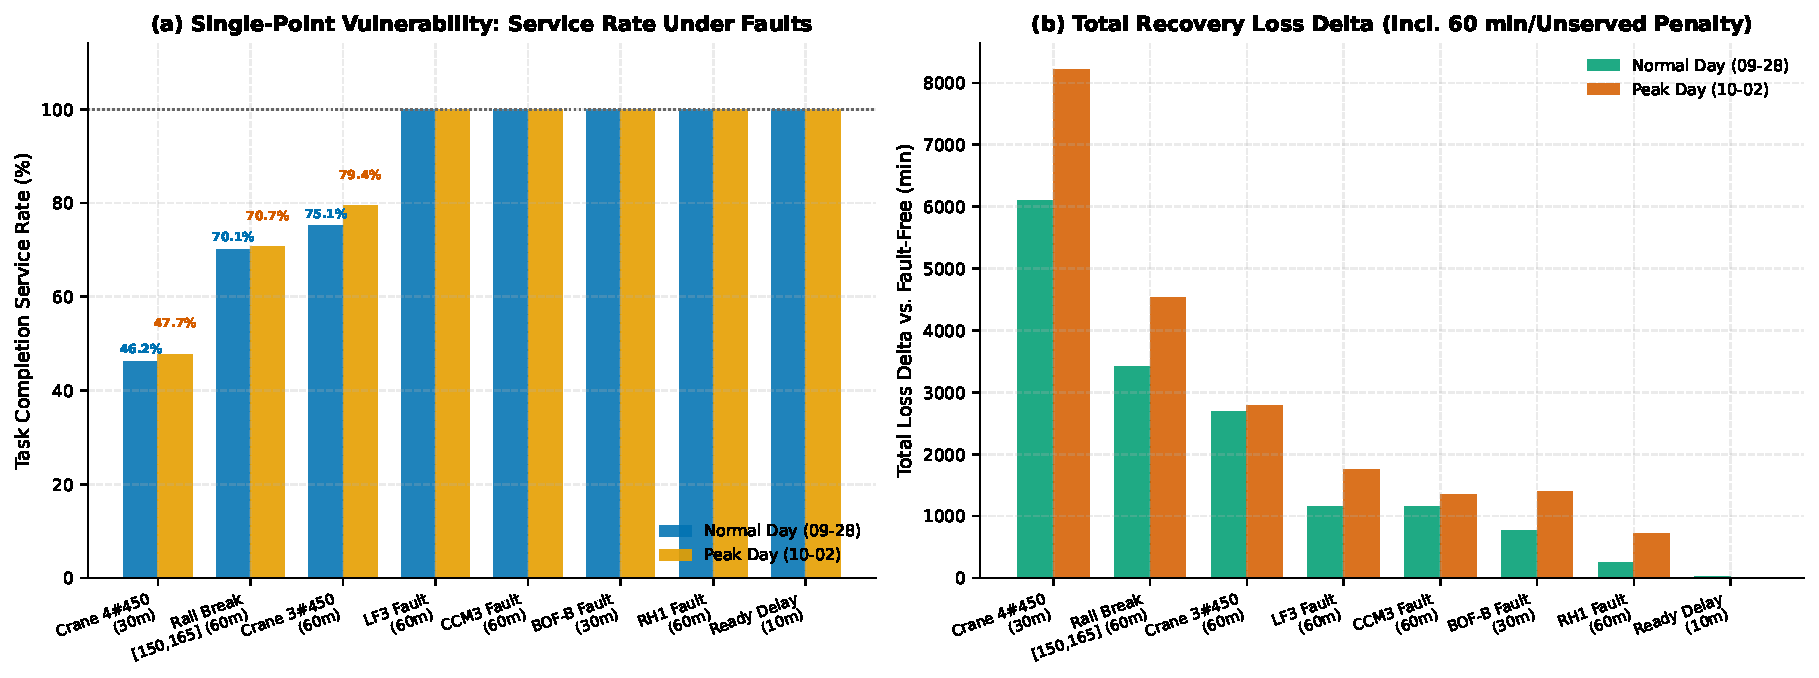
\includegraphics[width=0.96\textwidth]{figures/fig9_scene3_fault_recovery.pdf}
  \caption{(a) 8 类故障情景任务服务率对比；(b) 含未服务惩罚的总恢复损失增量。}
  \label{fig:scene3_faults}
\end{figure}

% ============================================================================
% 第七章：独立核验、消融与敏感性分析
% ============================================================================
\section{独立核验、消融与敏感性分析}
所有方案与轨迹均通过独立黑盒校验器与 \texttt{code/run\_all.py} 一键复现入口及 \texttt{pytest} 套件检验，全程 0 轨道碰撞；消融实验证实关闭主动避让在 \texttt{6C0754} 第 1 步即死锁，且均匀日块扰动下风险策略与均值派车差异有限。

% ============================================================================
% 第八章：钢厂调度管理建议、优势与局限
% ============================================================================
\section{钢厂调度员操作建议、优势与局限}

\subsection{致车间调度中心的实操备忘录}
\begin{enumerate}[leftmargin=1.5em,itemsep=2pt]
  \item \textbf{保持东侧平车集聚：} 峰值日将 \texttt{CART3} 西移至 90~m 使等待增加 996.1~min（+86.0\%），应优先维持东侧组团、避免空包回程侵入中区重包通道。
  \item \textbf{将 \texttt{4\#450} 列为首要巡检防线：} \texttt{4\#450} 停摆下服务率仅 46.2\%/47.7\%，建议对其及 $[150, 165]$~m 轨道段实施错峰预防性维护。
  \item \textbf{150~t 行车两端待命与例外启用：} 三台 450~t 主力运行，\texttt{1\#150/2\#150} 在两端（7.5/227~m）待命；仅在翻渣后正总吊重 $\le 145$~t 且外侧通道畅通时例外接管。
  \item \textbf{以实测事件滚动更新并监控热龄：} 相比静态计划，自适应滚动派车可减少 74.4\%--84.6\% 平均迟到；调度台应直接依据实测完工事件滚动重算并盯紧末道精炼至开浇热龄。
  \item \textbf{故障时优先 L1 保序，谨慎跨区替代：} 精炼设备短停时优先原路线等待，避免盲目跨跨调度导致热窗违约上升。
  \item \textbf{升级 MES 双主键关联：} 用 \texttt{(熔炼号, 钢包号)} + \texttt{临时罐号} 替代单熔炼号关联，根除 72 组重复熔炼号歧义。
\end{enumerate}

\subsection{模型优势与局限}
\textbf{优势：} 非破坏性数据取证；匀速折点防碰撞充要证明；覆盖四类完整 E--F 跨吊运任务；独立黑盒校验与一键复现。\\
\textbf{局限：} 米制尺度与运动参数属基于图 1 的工程标定初值；整日预约串行跨度略超 24~h 且当前场景 2/3 基于拟合期日块与持久障碍回放，动态修复解封与全并行整日优化为后续深化方向。

\newpage
\bibliographystyle{ieeetr}
\bibliography{refs}

\end{document}
